\documentclass{jsarticle}
%\usepackage{listings,jlistings}
\usepackage{multicol}
\usepackage{verbatim}
\usepackage{amsmath}
\usepackage[dvipdfmx]{graphicx}
\usepackage{mathrsfs}
\usepackage{bm}
\usepackage{braket}
%\makeatletter

%\def\@thesis{脳はいかに運動を制御するか}
%\def\id#1{\def\@id{#1}}
%\def\department#1{\def\@department{#1}}
%
%\def\@maketitle{
%\begin{center}
%{\huge \@thesis \par} %修士論文と記載される部分
%\vspace{10mm}
%{\LARGE\bf \@title \par}% 論文のタイトル部分
%\vspace{10mm}
%{\Large \@date\par}	% 提出年月日部分
%\vspace{20mm}
%{\Large \@department \par}	% 所属部分
%{\Large 学籍番号 \@id \par}	% 学籍番号部分
%%{\Large メールアドレス \@email \par}
%\vspace{10mm}
%{\large \@author}% 氏名 
%\end{center}
%\par\vskip 1.5em
%}
%
%\makeatother
%
%\title{レポート}
%\date{\today} 
%\department{理学部 物理・情報科学科 情報コース}
%\id{15-2202-021-1}
%%\email{v021de@yamaguchi-u.ac.jp}
%\author{北田 和}
%
%\begin{document}
%\maketitle
%\begin{center}
%\thanks{E-mailアドレス:v021de@yamaguchi-u.ac.jp}
%\end{center}
%\newpage

\title{腕の曲げ伸ばし運動を速く行う際の手首の動きの減少と上腕二頭筋、上腕三頭筋の筋活動量の増加}
\author{北田 和}



\begin{document}
%\center
%腕の曲げ伸ばし運動を速く行う際の手首、肘、肩関節の軌道と上腕二頭筋、上腕三頭筋の筋活動量への影響\\
\maketitle


\begin{abstract}

%バスケットボールでのキャッチ、野球の投球などの運動では
%スポーツで投げる動作を行った際に故障する
%球技ではなるべく速いボールを投げることが重要になることが多い。だが、
%特に速度に関して意識しなければ
%的に速く投げない限り、
%全速力で投げたボールより比較的ゆっくりとしたボールを投げる。
%意識していない場合に速いボールを投げることはできない。
%なぜボールを速く投げた方が良い
%ということを理解しているのに普段から全力で投げないのだろうか。
%のに全速力でボールを投げないのだろうか。
%なぜ、意識しない場合には速いボールではなく、ゆっくりとしたボールを投げてしまうのだろうか。
%そのためにはボールの速度に応じて、腕の曲げ伸ばし運動の速度を変える必要がある。では、上手く速度の調節が出来ない人はどのように練習すれば良いのだろうか。
%この原因を解明するために、腕を曲げ伸ばし運動に注目する。具体的には、
%腕の曲げ伸ばし運動を速くしようとする際の
%筋活動や、軌道への影響に注目する。
%腕の曲げ伸ばし運動を行なう際に速さをどのように制御しているのかを調べる。
%具体的には、
%手首、肘、肩関節の軌道と上腕二頭筋、上腕三頭筋の筋活動量を測定した状態で、
%このレポートではモーションキャプチャと筋電計を使用した測定結果を解析する流れを紹介するとともに、
%腕の曲げ伸ばし運動を何も指示を与えずにした場合となるべく速く動かすよう指示した場合を比較した。
%その結果、意識的に速く腕の曲げ伸ばし運動を行っている場合、腕へ負荷が何も指示を与えられなかった場合に比べて大きくなっている可能性が示唆された。
%ことで腕の曲げ伸ばし運動を速く行っている可能性が示唆された。
%が存在することが。
ボールを投げたり、楽器を叩いたりする場合など腕を速く動かすことはよくある。だが、よりボールを速く投げたり、楽器を速く叩いたりしたいと考えた場合、どうすれば良いのだろうか。これらに共通することとして、腕を速く動かすことが挙げられる。
%かしたいと思ったことはありませんか。
そこで、
%腕の動きのメカニズムを調べることで、より腕を速く動かす方法がわかるのではないかと考え、
腕の曲げ伸ばし運動に注目した。具体的には腕の曲げ伸ばし運動をする際に、何も指示されなかった場合となるべく速く動かすよう指示された場合の筋活動や関節の動きの変化を調べた。その結果、筋活動量の増加、腕を伸ばしきらない動きをすることで、腕の曲げ伸ばし運動を速くできることがわかった。
%とどのような関係を持つのでしょうか。
\end{abstract}


\section{序論}
ボールを投げたり、楽器を叩いたりする場合に腕を速く動かすことはよくある。そこで、「もっとボールを速く投げたい」、「もっと楽器を速く叩きたい」場合に重要となるのは、
%と考えたことがあると思います。
%これを実現するために、
%腕を速く動かすことが必要となります。
腕を速く曲げ伸ばしすることである。
では、腕を速く曲げ伸ばしするには
どのようにすれば良いのだろうか。
%ここで、腕を曲げ伸ばしする際
%メカニズムを調べることで、より腕を速く動かす方法がわかるのではないかと考えました。
%ボールを投げたり、キャッチしたり、カヌーを漕いだりするときなど、腕の曲げ伸ばし運動の速度を調節する機会はよく存在する。しかし、この速度の調節が上手く出来ない人はどのように練習すれば良いのだろうか。また、教える際にはどのように指導すれば良いのだろうか。
%球技では速い投球を行う必要がある。
%しかし、特に意識しなければ、
%だが、速く投球を行うことに注意しなければ速く投球することはできない。では、なぜ意識しなければ速い投球はできないのだろうか。
%この疑問を解決するために、私は投球に必要な腕の曲げ伸ばし運動に注目することにした。
%速い投球を行うためには腕の曲げ伸ばしを速くする必要がある。では、なるべく速く腕の曲げ伸ばし運動をした場合とそうでない場合には筋活動や関節の軌道に対し変化はあるのだろうか。\\
%この問題に当たって、腕を曲げ伸ばし運動の速度を調節する際に、遅い速度を調節するよりも、速い速度に調節を行うことの方が難しい。よって、人が腕を速く曲げ伸ばししようとする際の変化に注目することにした。\\
%手術によって刺入電極を埋め込みことによる測定や頭皮上電極、脳表電極による脳波の測定などが挙げられる。しかし、これらの信号は決して大きいものではなく、これによって得られる情報はどこに対する何をするための信号であるかはわからない。そこで、脳の指令が比較的大きくでる筋電位から脳が筋肉に送る信号を観察することで、脳の働きを間接的に調べることができる。\\
% このレポートでは、脳が実際に筋肉を使用してどのように運動の速度を制御しているのかを考察することが目的である。計測実験では腕の曲げ伸ばし運動における筋電位と座標位置の変化を測定し、何も考えずに腕の曲げ伸ばしを行った際となるべく速く行った際の違いをみる。これにより、脳が筋肉に送る速度についての信号がどのように変化しているかを調べる。\\
そこで、被験者に腕の曲げ伸ばし運動を何も指示をせずに行ってもらう場合(slow-task)となるべく速く行うよう指示した場合(fast-task)の2通りの計測実験を行うことにし、上腕二頭筋と上腕三頭筋の筋電と手首、肘、肩の座標を測定し、fast-taskに対する筋活動量と関節の座標がどのように変化するかを調べた。


%もっと具体的に
\section{手法}
被験者(19歳、男性、陸上部所属)に机に利き腕を置いて腕の曲げ伸ばし運動をするように指示した。図\ref{karada1}にこの際のイメージを示す。測定計は、ワイヤレス筋電センサ 乾式・加速度16G[LP-WS1222]を上腕二頭筋、上腕三頭筋の二カ所に、モーションキャプチャ用の反射マーカを図\ref{karada2}のイメージのように手首、肘、肩に取り付けた。モーションキャプチャのカメラは被験者の頭上から撮影し、腕の曲げ伸ばし運動を二次元平面として捉えた。この平面の次元軸は図のとおりである。この際に撮影の関係上、被験者には膝立ちで机に向かってもらった。なお、筋電センサはサンプリング周波数1000Hzで測定を行った。
%付属している加速度センサに関しては、
今回はモーションキャプチャによる関節の軌道に注目したため、付属している筋電センサは使用していない。\\
 普通に腕の曲げ伸ばし運動を行う場合と速く曲げ伸ばし運動を行うことを意識する場合を比較するため、被験者に対し何も指示を出さず腕の曲げ伸ばし運動を行った場合(slow-task)となるべく速く腕の曲げ伸ばし運動を行うように指示した場合(fast-task)を測定する二回の計測実験を行った。\\
 実験一回の計測時間は20秒間に設定した。
また、腕の曲げ伸ばしを開始して約5秒後から計測を開始することで、腕の曲げ伸ばし運動をしているデータのみを取得した。

%のデータを計測することで、すべてのデータが腕の曲げ伸ばし運動を行っているものを取得できるようにした。
\begin{figure}[htb]
\begin{center}
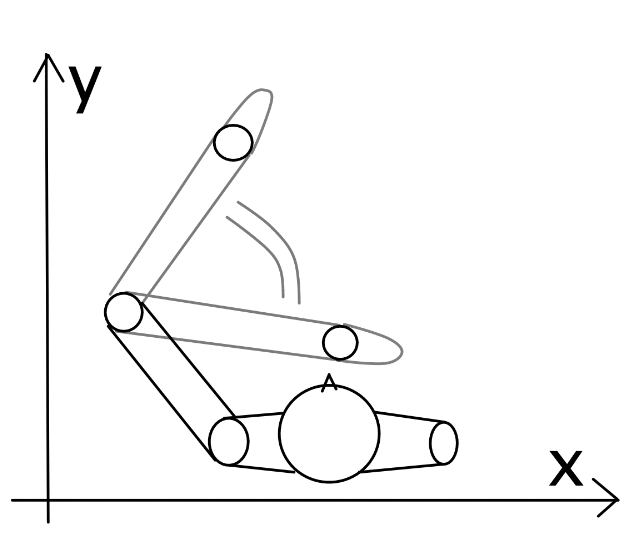
\includegraphics[width=5cm]{karada1.png}
\caption{腕の曲げ伸ばし運動のイメージ}
\label{karada1}
\end{center}
\end{figure}

%細かい装置の説明はいらない
%あたりまえのことから
%空間ではない
%何度も聞き落とすと相手にされなくなるから
%早く書く
%時が経っても覚えてるように

%\subsection{計測方法}
%筋電計は上腕二頭筋と上腕三頭筋の二カ所に、反射マーカは肩、肘、手首関節の三カ所に取り付けた。(図\ref{karada2}参照)筋電計はワイヤレス乾式のものを使用し、筋電位を測定できるところでテープで固定した。反射マーカは光を受けた方向に反射するものであり、モーションキャプチャ用の撮影カメラの近くに白熱灯をつけ、反射した光がカメラに映るように設置する。この反射した光をトラッカーとして使用し、モーションキャプチャを行った。この際のカメラは被験者の頭上から撮影し、腕の動きを二次元空間として捉えた。
\begin{figure}[htb]
\begin{center}
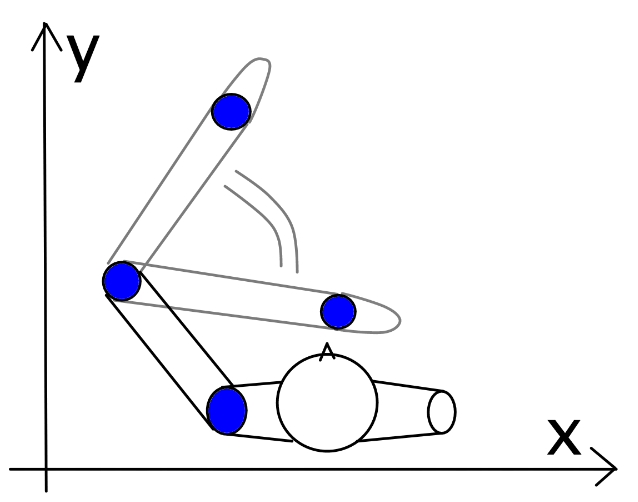
\includegraphics[width=5cm]{karada.png}
\caption{モーションキャプチャの反射マーカ貼り付け位置イメージ}
\label{karada2}
\end{center}
\end{figure}


\subsection{筋電データ処理}
筋活動の変化に注目するため、1$\sim$4Hzの通過領域をもつバンドパスフィルタをかけることで、
筋電計から取得したデータに混じる高周波のノイズを除去した。
%筋活動の変化に注目するため、pythonで1$\sim$40Hzをバターワースフィルタを用いたバンドパスフィルタによって取り出した。
この際、全体の時間のずれを直すためfiltfiltをかけた。
次に、筋肉の活動度を時間変化として比較するため、(\ref{s2})の式を用いて$\Delta T$間の筋活動量を算出した。以上の処理を行うプログラムを\ref{prog1}にまとめた。



\begin{equation}
a(t)=\frac{1}{\Delta T}\int_{t-\Delta T/2}^{t+\Delta T/2}|E(t)|dt 
\label{s2}
\end{equation}


\subsection{モーションキャプチャデータ処理}
得られたデータには、ヘッダ部に計測点数、単位時間当たりのコマ数などの情報があり、テール部には最小値、最大値などの情報が含まれている。また、データ部にはシーン、時間、座標Xの各計測点データ、座標Yの各計測点データが含まれている。しかし、この時間データは10ms刻みであるため、得られた座標データの時間よりも大まかである。そのため、ヘッダ部の単位時間当たりのコマ数から座標データに対応する細かな時間を求めて解析に使用した。以上の処理を行うプログラム\ref{prog2}にまとめた。


\section{Results(結果)}
図\ref{tym3}に被験者のy軸方向の手首の座標変化を計測開始時間から1$\sim$4秒の3秒間のデータを元に作成したグラフを掲示する(今後、説明がない場合はslow-taskの結果を青、fast-taskの結果を赤のグラフで示す。)。この図より、y軸方向にslow-taskが3回、fast-taskが7回手首を前後させていることが示される。\\
\begin{figure}[htb]
\begin{center}
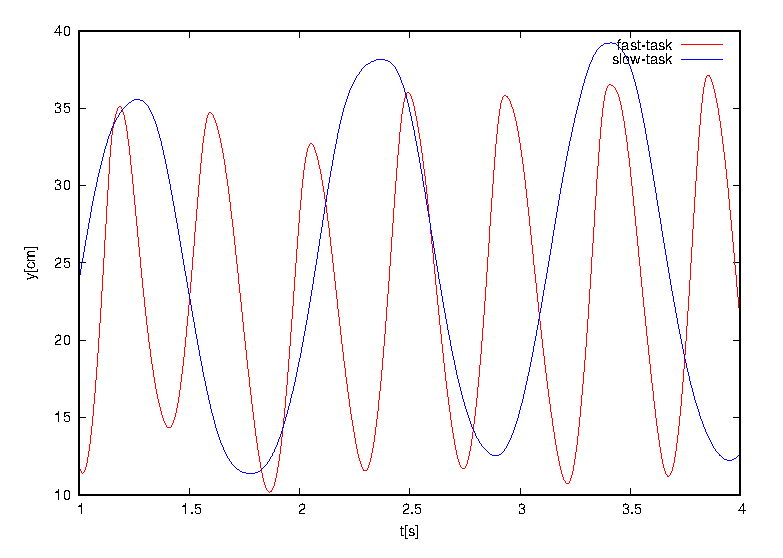
\includegraphics[width=10cm]{tym3.eps}
\caption{手首の時間におけるy軸方向の動き}
\label{tym3}
\end{center}
\end{figure}


%\newpage
ここで、図\ref{tym3}と同時間の上腕二頭筋、上腕三頭筋のEMG活動量のデータをグラフにした図\ref{kkdata1}、\ref{kkdata2}に注目する。図\ref{kkdata1}のfast-taskでは1.6秒に、slow-taskでは2.3秒に活動量のピークが存在する。一方、図\ref{tym3}のfast-taskでは1.6秒に、slow-taskでは2.4秒に手首がy軸の正の方向に出るタイミング存在する。これは、上腕二頭筋の活動量のピークと手首がy軸の正の方向に出るタイミングがほぼ等しいことがこれ以外にも同様に存在するため、主に腕を伸ばすタイミングに上腕二頭筋を使用していることが示唆される。また、同様に、図\ref{kkdata2}のfast-taskでは1.8秒に、slow-taskでは2.7秒に活動量のピークが存在する。一方、図\ref{tym3}のfast-taskでは1.8秒にslow-taskでは2.8秒に手首がy軸の負の方向に戻るタイミング存在する。このように、上腕三頭筋の活動量のピークと手首がy軸の負の方向に戻るタイミングがほぼ等しいことがこれ以外にも同様に存在するため、主に腕を曲げるタイミングに上腕三頭筋を使用していることが示唆される。\\
 次に、純粋な筋活動の特徴としては、
%どちらの筋活動量も滑らかな山を描くわけではなく、上がったり下がったりを繰り返しながら変動をしている。また、
上腕二頭筋のfast-taskでは1.6秒に、slow-taskでは2.3秒に筋活動量のピークが存在することは前述したが、その後fast-taskでは1.8秒に、slow-taskでは2.7秒に筋活動量は下がっている。同様の傾向がその他にも存在する。一方、上腕三頭筋のfast-taskでは1.8秒に、slow-taskでは2.7秒に筋活動量のピークが存在し、その後fast-taskでは2.1秒に、slow-taskでは3.1秒に小さなピークが存在し、同様の傾向がその他にも存在する。これは、腕の曲げ伸ばしに対して上腕二頭筋は腕を伸ばすタイミングで収縮させているが、上腕三頭筋は腕を曲げるタイミングと伸ばすタイミングどちらでも収縮させていることを現している。\\


\begin{figure}[htb]
\begin{center}
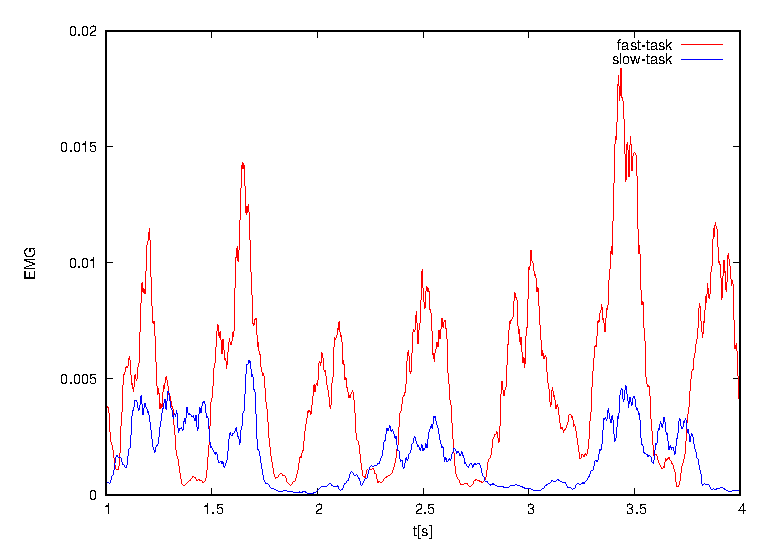
\includegraphics[width=10cm]{kkdata1.eps}
\caption{上腕二頭筋のEMG活動量}
\label{kkdata1}
\end{center}
\end{figure}


\begin{figure}[htb]
\begin{center}
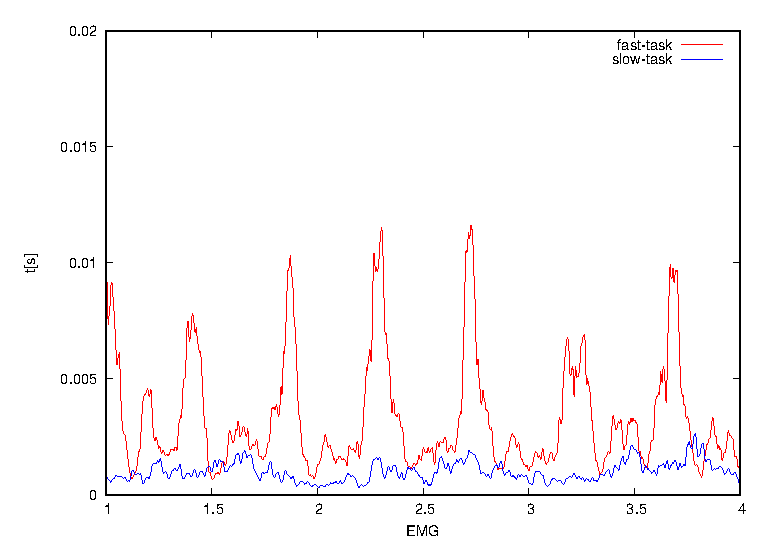
\includegraphics[width=10cm]{kkdata2.eps}
\caption{上腕三頭筋のEMG活動量}
\label{kkdata2}
\end{center}
\end{figure}


\newpage
そこで、図\ref{hikaku1}、図\ref{hikaku2}に上腕二頭筋、上腕三頭筋のそれぞれのEMG活動量のグラフと被験者の正面方向の手首の座標変化を重ねたグラフを示す。
%上腕二頭筋が図\ref{hikaku1}、上腕三頭筋が図\ref{hikaku2}のようになった。
%この際、関係を見やすくするために筋活動量を上腕二頭筋を2000倍、上腕三頭筋のfastを3000倍、slowを15000倍している。
これより、上腕二頭筋では腕を伸ばしたタイミングより活動量増加のピークは若干遅く起こる傾向があった。また、上腕三頭筋では腕を曲げ終わるタイミングよりも前に活動量増加のピークが起こる傾向があった。\\
\begin{figure}[htb]
\begin{center}
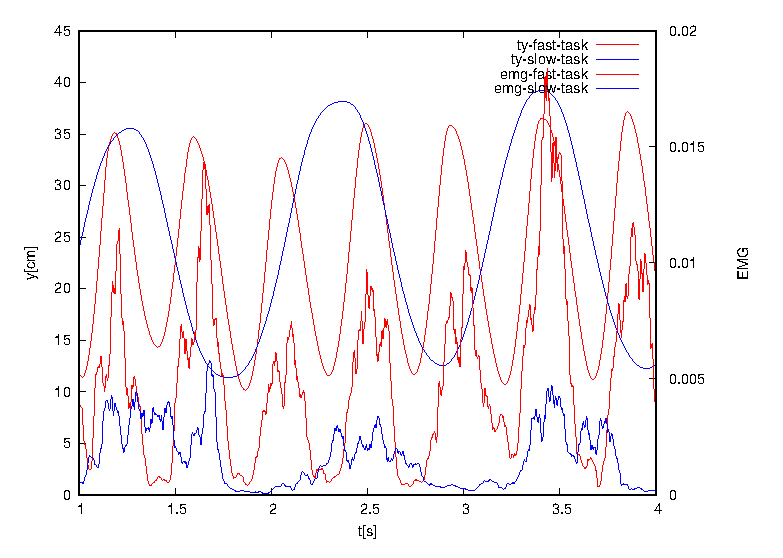
\includegraphics[width=10cm]{hikakudata1.eps}
\caption{上腕二頭筋のEMG活動量と手首の動きの比較}
\label{hikaku1}
\end{center}
\end{figure}

\begin{figure}[htb]
\begin{center}
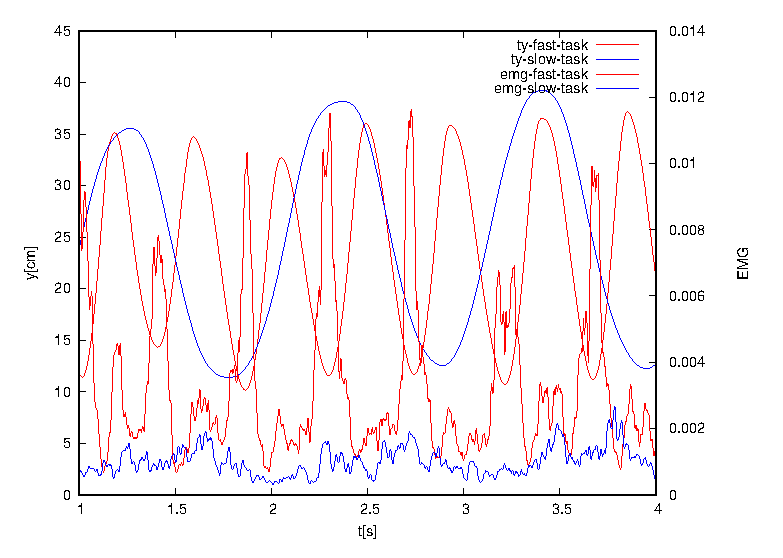
\includegraphics[width=10cm]{hikakudata2.eps}
\caption{上腕三頭筋のEMG活動量と手首の動きの比較}
\label{hikaku2}
\end{center}
\end{figure}


\newpage
次に、slow-taskとfast-taskの比較を行う。筋活動に注目するとslow-taskとfast-taskでは上腕二頭筋でも上腕三頭筋でもfast-taskの筋活動量の方が多くなっている。これより、腕の曲げ伸ばし運動を速く行おうと意識した方が、筋活動量が多くなる傾向がある。では筋活動量の変動には大きな変化は見られるのだろうか、ここで、手首のy軸方向の動きに対しての筋活動量の変化を見るために腕を曲げた状態から腕を3往復させた分のデータを取り出し比較する。図\ref{hikaku3}、図\ref{hikaku4}に時間をslow-taskが約0.7$\sim$4.0秒、fast-taskが約1.4$\sim$2.7秒のデータを切り出し時間に対して正規化した結果と対応する上腕二頭筋、上腕三頭筋の筋活動量をそれぞれグラフ化したものを示す。
\begin{figure}[htb]
\begin{center}
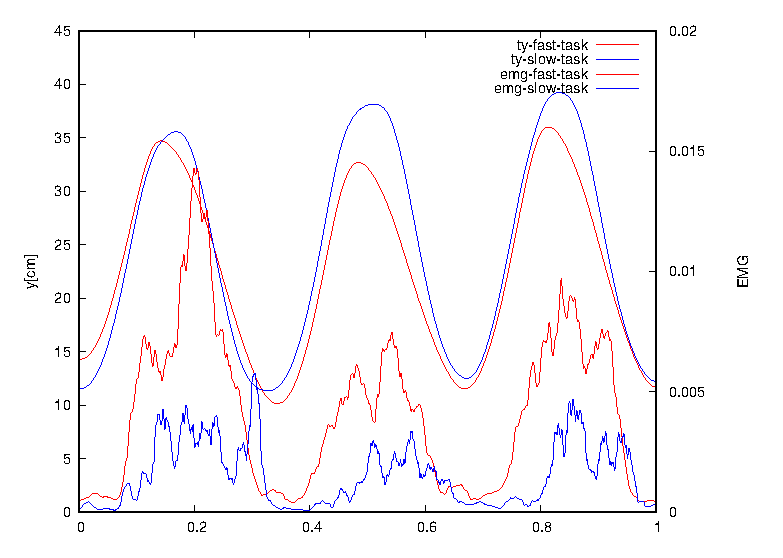
\includegraphics[width=10cm]{hikakudata3.eps}
\caption{正規化後の上腕二頭筋のEMG活動量と手首の動きの比較}
\label{hikaku3}
\end{center}
\end{figure}

\begin{figure}[htb]
\begin{center}
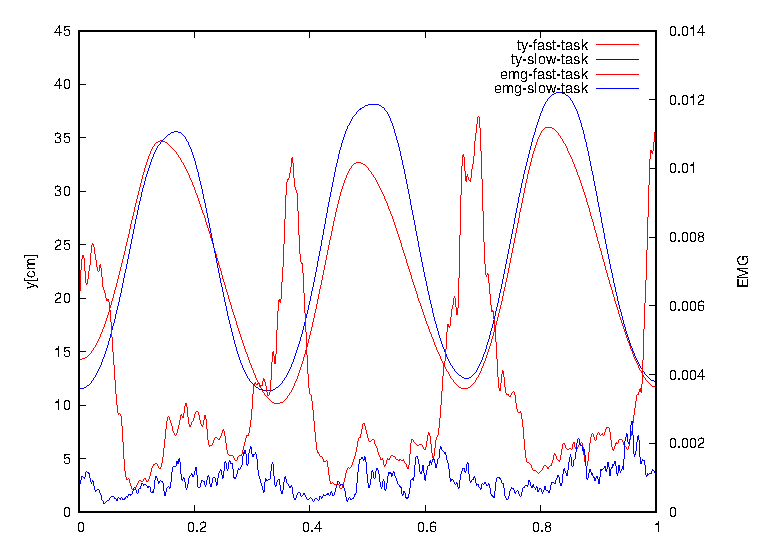
\includegraphics[width=10cm]{hikakudata4.eps}
\caption{正規化後の上腕三頭筋のEMG活動量と手首の動きの比較}
\label{hikaku4}
\end{center}
\end{figure}



\newpage
まず、手首のy軸方向の前後の軌道について注目するとslow-taskに対して、fast-taskの方が3$\sim$4cmほど前後が小さくなっていることが示される。また、slow-taskは腕の曲げる速度も伸ばす速度も大体等しいのに対して、fast-taskは腕を伸ばすときの速度の方が曲げる速度よりも速くなっていることが示される。
次に、筋活動に注目する。上腕二頭筋では大きな差は見られないのに対し、上腕三頭筋ではslow-taskは腕が曲がりきる前に筋活動量のピークが来ているのに対して、fast-taskは腕が曲がりきった後に筋活動量のピークが来ていることが示される。




\section{Discussion(考察)}
fast-taskでは筋活動量が増加したことより、
%として、fast-taskの方がより筋肉を使用していることが分かったため、
筋肉量をあげれば腕を速く曲げ伸ばしできることが考えられる。また、fast-taskではy軸方向の手首の動きが減少したことより、
%fast-taskの方がy軸方向の動きが小さくなっていることが分かったため、
小さく曲げ伸ばし運動をすれば腕を速く曲げ伸ばしできることが考えられる。以上のことにより、楽器を叩く場合などのような伸ばしきる必要がない場合には腕をなるべく小さく曲げ伸ばしできるように練習することで、
%速く動かすことができると考えた。
伸ばしきる必要がある場合にも共通しては、
筋肉を鍛えることで速く動かすことができると考えられる。
%一方、ボールを投げる場合などのような伸ばしきる必要
%まず、
%上腕二頭筋と上腕三頭筋で筋活動量の時間変化に違いが生まれた原因を腕の動きを力学的に捉え考える。肘関節の角速度$\omega$を腕伸ばす方向を正、曲げる方向を負として定義する(図\ref{omega}参照)。
%\begin{figure}[htb]
%\begin{center}
%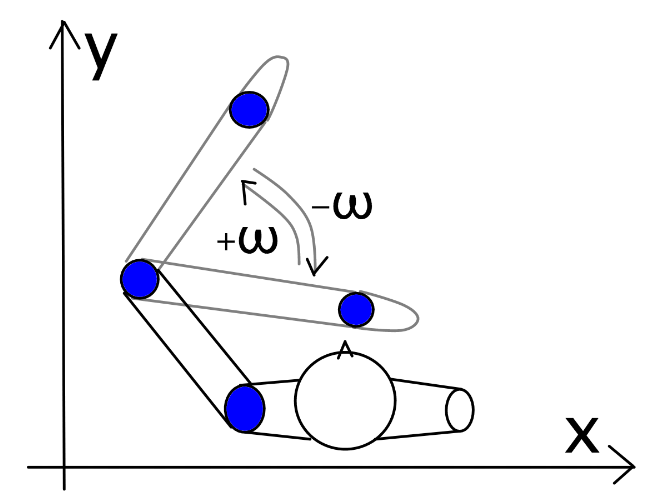
\includegraphics[width=7cm]{omega.png}
%\caption{肘関節の角速度の定義}
%\label{omega}
%\end{center}
%\end{figure}
%
%ここで、腕の曲げ伸ばし運動のタイミングと$\omega$の関係を表\ref{ot}のようになる。なお、$\omega\rightarrow+0$は$\omega$が正から0になることを示す。
%\begin{table}[htb]
%\begin{center}
%\caption{腕の動きと$\omega$の関係}\label{ot}
%\begin{tabular}{| l | l |}\hline
%腕を伸ばしている間 & $\omega>0$\\ \hline
%腕を伸ばしきった時 & $\omega=0(\omega\rightarrow+0)$\\ \hline
%腕を曲げている間 & $\omega<0$\\ \hline
%腕を曲げきった時 & $\omega=0(\omega\rightarrow-0)$\\ \hline
%\end{tabular}
%\end{center}
%\end{table}
%
%次に、上腕二頭筋と上腕三頭筋はそれぞれ、図\ref{kin}のような位置に存在する。よって、上腕二頭筋が収縮すれば$\omega<0$の力が、上腕三頭筋が収縮すれば$\omega>0$の力が働く。
%\begin{figure}[htb]
%\begin{center}
%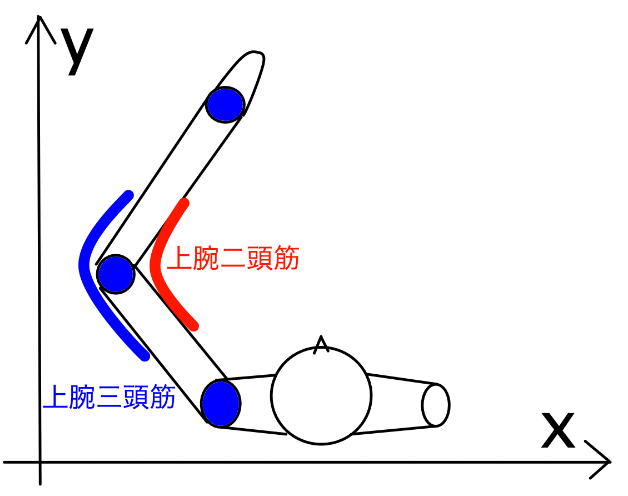
\includegraphics[width=7cm]{kin.png}
%\caption{上腕二頭筋と上腕三頭筋の位置}
%\label{kin}
%\end{center}
%\end{figure}


%$$\omega\rightarrow 0\rightarrow-\omega\rightarrow0\rightarrow\omega\rightarrow\dots$$
%と変動しており、$\omega$のタイミングで腕を伸ばし、

%なぜ筋活動量のグラフではなぜ上がったり下がったりを繰り返しているのかであるが、脳は発火の頻度を変えることで筋肉の収縮度を調節している。このため、発火が少なければ、発火を多くすれば筋肉はより強く
%y軸方向の手首の軌道のピークと筋活動量のピークにはなぜずれが生じたのだろうか、

%なぜ実際の動きと筋活動量のピークにはずれが生じたのだろうか、この原因には2つの可能性が挙げられる。まず、モーションキャプチャと筋電計の測定時間がずれている可能性がある。しかし、これは、2つの筋電計がどちらも同じ時間方向へのずれならば高い可能性を持つが、今回の結果では、上腕二頭筋では遅れ、上腕三頭筋では速くずれているため可能性が低いのではないかと考えた。\\

%ここで、体を保護するためという可能性がある。
%以上のことにより、上腕二頭筋では腕を伸ばしたタイミングより活動量増加のピークは若干遅く起こる傾向があったことを考える。
%腕を伸ばしきるには$\omega>0$から$\omega=0$と変化させる必要がある。また、腕を曲げ始めるには$\omega=0$から$\omega<0$と変化させる必要がある。
%そのためには、$\omega<0$の力を加えればよいため、上腕二頭筋が働いたのではないかと考えられる。
%また、活動量増加のピークが伸ばしたタイミングより活動量増加のピークが若干遅く起こっ
%ここで、筋活動量増加のピークがなぜ腕を伸ばしたタイミングより後に存在するかを考える。腕が伸びきった時は肘関節の可動領域の限界であるため、関節を使用して$\omega=0$になるようにしている可能性が挙げられる。
%$\omega=0$から$\omega<0$よりも考えられ、この際、腕を。%腕を伸ばしきったタイミングで$\omega=0$であるため、

%同様に、上腕三頭筋では腕を曲げ終わるタイミングよりも前に活動量 増加のピークが起こる傾向があったことを考える。
%腕を曲げきるには$\omega<0$から$\omega=0$と変化させる必要がある。また、腕を伸ばし始めるには$\omega=0$から$\omega<0$と変化させる必要がある。
%そのためには、$\omega>0$の力を加えればよいため、上腕三頭筋が働いたのではないかと考えられる。
%ここで、なぜ筋活動量増加のピークがslow-taskとfast-taskで腕を曲げる前と曲げた後にピークが存在するかを考える。
%腕を曲げきった状態から



%これらを踏まえてslow-taskとfast-taskの変化として、腕に対する負荷を上げることで腕の曲げ伸ばしを速くしており、意識的に腕の曲げ伸ばしを速くしていないslow-taskの場合には腕に対し負荷が少なくなるようにしているのではないかと考えた。
%根拠としては、腕を伸ばす際には関節で腕の伸びが止まった後にさらに$\omega>0$の力が加われば、肘関節に負担がかかりそのまま関節が外れてしまう。そのため、腕が伸びきったところで、腕を伸びようとする力を抑えるために上腕二頭筋が活動している。
%ここで、slow-taskの場合$\omega$の値も小さく、肘関節が伸びきった後にかかる負荷も少ないため、上腕二頭筋の筋活動量も小さくなる。一方、fast-taskの場合$\omega$の値は大きく、肘関節が伸びきった後にかかる負荷も大きいため、上腕二頭筋の筋活動量も大きくなるといえる。
%
%次に、腕を曲げる場合、最後まで腕を曲げきると拳が肩や胸に当たってしまう。そこで、slow-taskの場合は腕が完全に曲がり拳が当たる前に腕を曲げる力を抑えるために上腕三頭筋が活動しており、逆にfast-taskの場合はその制御を外すことにより速く腕の曲げ伸ばしを行うことができる。以上により、結果のグラフの説明がつくため、この可能性が有力ではないかと考えられる。
%
%これを確かめるためには、拳を肩や胸にぶつけて腕の曲げ伸ばし運動を行う実験や筋活動が腕の曲げ伸ばし運動の直後で上がらない運動を行った際のシミュレーションを行いどのくらいの負荷が体にかかるかを調べるなどが挙げられる。




\section{Conclusions(結論)}
腕の曲げ伸ばし運動を行う際には大まかに伸ばす時に上腕二頭筋を曲げる時に上腕三頭筋を使用している。しかし、それぞれの活動量のピークは上腕二頭筋は腕を伸ばし終わった後に、上腕三頭筋はslow-taskの際は腕を曲げ終わる直前に、fast-taskの際は腕を曲げ終わった後にある。

\newpage
\appendix

\section{筋電データの処理のプログラム\label{prog1}}
\subsection{バンドパスフィルタのプログラム}
\begin{multicols}{2}
\scriptsize
\begin{verbatim}
     1	import csv
     2	import numpy as np
     3	from scipy import signal
     4	import matplotlib.pyplot as plt
     5	%matplotlib inline
     6	import pandas as pd
     7	from pandas import Series, DataFrame
     8	
     9	f = open('PID255_MID11_FileID002_000000_0010.csv',
     'r',encoding="shift-jis")
    10	s = open('data_12_2.txt','w',encoding="shift-jis")
    11	i=0
    12	datam=''
    13	dataReader = csv.reader(f)
    14	
    15	t, emg, x, y, z= [], [], [], [], [] 
    16	
    17	for row in dataReader:
    18	    if i<10:
    19	        datam=datam+str(row)
    20	    else:
    21	        s.writelines('%s\n' %("   ".join(row)))
    22	        t += [float(row[0])]
    23	        emg += [float(row[1])]
    24	        x += [float(row[2])]
    25	        y += [float(row[3])]
    26	        z += [float(row[4])]
    27	
    28	    i=i+1
    29	 
    30	print(datam)
    31	f.close()
    32	s.close()
    33	
    34	n = i-10
    35	dt =0.001
    36	f = 1000
    37	fn = 1/(2*dt)
    38	td = np.linspace(1, n, n)*dt-dt
    39	
    40	fp = 1
    41	fs = 40
    42	kagen = 0.01
    43	jougen = 1.0
    44	
    45	Wp = fp/fn
    46	Ws = fs/fn
    47	
    48	N, Wn = signal.buttord(Wp, Ws, kagen, jougen)
    49	b1, a1 = signal.butter(N,Wn, "low")
    50	y1 = signal.filtfilt(b1, a1, emg)
    51	
    52	plt.figure()
    53	plt.plot(td, emg, "b")
    54	plt.plot(td, y1, "r", linewidth=2 , label="butter")
    55	plt.xlim(0,1)
    56	plt.xlabel("Time [s]")
    57	plt.ylabel("Amplitube");
    58	
    59	x=0
    60	ef = open('bandpass11_1.txt','w',encoding="shift-jis")
    61	while x < n:
    62	    ef.write('%f,' %td[x])
    63	    ef.write('%f\n'  %y1[x])
    64	    x+=1
\end{verbatim}
\normalsize
\end{multicols}

\subsection{整流化のプログラム}
\begin{multicols}{2}
\scriptsize
\begin{verbatim}
     1	#include<stdio.h>
     2	#include<math.h>
     3	int main(void){
     4	  FILE *rf, *wf;
     5	  double data[2];
     6	  
     7	  rf = fopen("bandpass12_2.txt","r");
     8	  wf = fopen("abs12_2.txt","w");
     9	  
    10	  while((fscanf(rf,"%lf,%lf",&data[0],&data[1]))!=EOF){
    11	    fprintf(wf,"%f,%f\n",,data[0],fabs(data[1]));
    12	  }
    13	  
    14	  return 0;
    15	}
\end{verbatim}
\normalsize
\end{multicols}

\subsection{活動量の変化を求めるプログラム}
\begin{multicols}{2}
\scriptsize
\begin{verbatim}
     1	#include<stdio.h>
     2	#include<stdlib.h>
     3	#include<math.h>
     4	#define BUF_SIZE 256
     5	#define DT 50
     6	#define SAMPLE 1000
     7	void integration(double e[],double a[], int n){
     8	  int i;
     9	  for(i=0; i<DT; i++){
    10	    a[0]+=(e[i]/SAMPLE);
    11	  }
    12	  for(i=1; i<(n-DT); i++){
    13	    a[i]=a[i-1]+(e[i+DT]-e[i-1])/SAMPLE;
    14	  }
    15	}
    16	
    17	/*------------------------------------------------*/
    18	int main(void){
    19	  FILE *rf, *wf;
    20	  double data, *e, *a;
    21	  int n=0, i;
    22	  char buf[BUF_SIZE];
    23	  
    24	  if((rf = fopen("abs12_2.txt","r")) ==NULL)
    25	    return -1;
    26	  wf = fopen("katudou12_2.txt","w");
    27	  
    28	  while((fgets(buf,BUF_SIZE,rf))!=NULL){
    29	    n++;
    30	  }
    31	
    32	
    33	  fclose(rf);
    34	  if((rf = fopen("abs12_2.txt","r")) ==NULL)
    35	    return -1;
    36	  
    37	  e =(double*)malloc(sizeof(double)*n);
    38	  a =(double*)malloc(sizeof(double)*(n-DT));
    39	  
    40	  if(e == NULL || a == NULL){
    41	    printf("メモリが確保できませんでした。\n");
    42	    exit(EXIT_FAILURE); 
    43	  }
    44	  
    45	  for(i=0; i<(n-DT); i++)
    46	    a[i]=0;
    47	  
    48	  i=0;
    49	  while((fscanf(rf,"%lf ,",&data))!=EOF){
    50	    fscanf(rf,"%lf",&e[i]);
    51	    i++;
    52	  }
    53	
    54	  integration(e,a,n);
    55	
    56	  
    57	  for(i=0; i<(n-DT); i++)
    58	    fprintf(wf,"%lf,%lf\n",((double)(i+(DT/2))/1000.0),a[i]);
    59	  
    60	  
    61	  fclose(rf);
    62	  free(a);
    63	  free(e);
    64	  fclose(wf);
    65	  
    66	  return 0;
    67	}
\end{verbatim}
\normalsize
\end{multicols}


\section{モーションキャプチャデータの処理のプログラム\label{prog2}}
\subsection{データをデータ部とそれ以外に分けるシェルスクリプト}
\scriptsize
\begin{verbatim}
     1	#!/bin/bash
     2	if test ! -e $1.csv && test ! -e $1; then
     3	    echo "ファイルを指定してください"
     4	elif test -f $1.csv; then
     5	#    FNAME="$1"
     6	    nkf -w $1.csv |sed -E "s_^,//g"| sed -E "s/^[\t ]+//g" | egrep "^[0-9]"  > pos-$1.dat
     7	    nkf -w $1.csv | sed "s/,/ /g" | sed -E "s/^[\t ]+//g" | egrep -v "^[0-9]"  > info-$1.dat
     8	else
     9	    nkf -w $1 |sed -E "s_^,//g"| sed -E "s/^[\t ]+//g" | egrep "^[0-9]"  > pos-${1/.csv/}.dat
    10	    nkf -w $1 | sed "s/,/ /g" | sed -E "s/^[\t ]+//g" | egrep -v "^[0-9]"  > info-${1/.csv/}.dat 
    11	fi
\end{verbatim}
\normalsize



\subsection{データ部をマーカごとにファイル分けするプログラム\label{prog3}}
\begin{multicols}{2}
\scriptsize
\begin{verbatim}
     1	#include<stdio.h>
     2	#include<stdlib.h>
     3	#include<string.h>
     4	#include<math.h>
     5	#define N 20
     6	#define M 256
     7	int main(int argc,char *argv[]){
     8	  FILE *rf,*wf[N];
     9	  double sample, *data;
    10	  int makar, i=0,n=1, dmen;
    11	  char fn[N][M]={'\0'};
    12	  
    13	  
    14	  if( (sample = atof(argv[1]))==0 || 
    (makar = atoi(argv[2])) ==0 || (dmen = atoi(argv[3]))==0 ){
    15	    printf("サンプリング周波数、マーカ数を数値で入力してください。\n\a");
    16	    i=-1;
    17	  }
    18	  else if((rf = fopen(argv[4],"r"))==NULL){
    19	    printf("ファイルが存在しません。\n\a");
    20	    i=-1;
    21	  }
    22	  if(i==-1){
    23	    printf("extract <サンプリング周波数> <マーカ数> <次元> <ファイル名>\nで指定してください。\n");
    24	    return 0;
    25	  }
    26	  
    27	  
    28	  
    29	  for(i=0; i<makar; i++){
    30	    sprintf(fn[i],"%d-%s",(i+1),argv[4]);
    31	    wf[i]=fopen(fn[i],"w");
    32	  }
    33	  
    34	  data = malloc(sizeof(double)*(dmen*makar+2));
    35	  
    36	  while(fscanf(rf,"%lf ,%lf ",&data[0],&data[1])!=EOF){
    37	    
    38	    for(i=0; i<(makar*dmen); i++){
    39	      if( ( fscanf(rf,",%lf ",&data[i+2]))==EOF ){
    40		printf("元ファイルに欠損があります。
    出来たファイルは使えません。\n");
    41		return 0;
    42	      }
    43	    }
    44	    
    45	    for(i=0; i<makar; i++){
    46	      fprintf(wf[i],"%lf",data[0]/sample);
    47	    }
    48	    
    49	    for(i=0; i<(dmen*makar); i++)
    50	      fprintf(wf[i%makar],",%lf",data[i+2]);
    51	    for(i=0; i<makar; i++)
    52	      fprintf(wf[i],"\n");
    53	  }
    54	  
    55	  
    56	  fclose(rf);
    57	  for(i=0; i<makar; i++)
    58	    fclose(wf[i]);
    59	  
    60	  free(data);
    61	  
    62	  return 0;
    63	}
\end{verbatim}
\normalsize
\end{multicols}



\subsection{ヘッダ部から情報を取り出し\ref{prog3}に数値を与えるシェルスクリプト}
\scriptsize
\begin{verbatim}
     1	#!/bin/bash
     2	if test ! -e $1.csv && test ! -e $1; then
     3	    echo "ファイルを指定してください"
     4	elif test -f $1.csv; then
     5	    ./extract $(grep "コマ数" info-$1.dat  |cut -f 1 -d "/"|sed "s/[^0-9|.]//g") 
     $(grep "計測点数" info-$1.dat  |cut -f 2 -d "," | grep -o [0-9]) 2 pos-$1.dat
     6	else
     7	    ./extract $(grep "コマ数" info-${1/.csv/}.dat  |cut -f 1 -d "/"|sed "s/[^0-9|.]//g") 
     $(grep "計測点数" info-${1/.csv/}.dat  |cut -f 2 -d "," | grep -o [0-9]) 2 pos-${1/.csv/}.dat
     8	fi
\end{verbatim}
\normalsize


\subsection{入力ファイルの座標データのみをファイル出力するシェルスクリプト}
\scriptsize
\begin{verbatim}
     1	#!/bin/bash
     2	if test ! -e $1.dat && test ! -e $1; then
     3	    echo "ファイルを指定してください"
     4	elif test -f $1; then
     5	    cut -f 2- -d "," $1 |  sed -e 's/^[ ]*//g' > ${1/pos/xy}
     6	else
     7	    cut -f 2- -d "," $1.dat | sed -e 's/^[ ]*//g' > ${1/pos/xy}.dat
     8	fi
\end{verbatim}
\normalsize



%\begin{figure}[htb]
%\begin{center}
%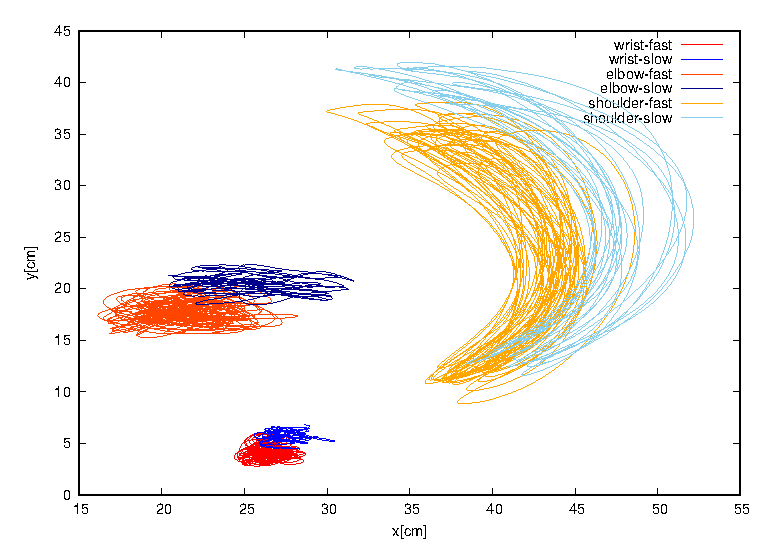
\includegraphics[width=10cm]{xym1.eps}
%\caption{全体の動きの時間変化}
%\label{xym1}
%\end{center}
%\end{figure}
%
%
%
%\section{筋電データの処理}
%それぞれのプログラム文は以下のようになった。
%\subsection{筋電位に1$\sim$40Hzの通過帯域を持つバンドパスフィルター(3次バターワース)をかける。ただし、単純にバンドパスフィルターをかけるとデータのピーク位置が実際の時刻より少し遅くなることが多い。そこで、順方向と逆方向の両方から一回ずつフィルター処理をすることで時間的なズレを補正する。この処理は、pythonならばscipyのfitfit関数を使えば自動で行われる。}\label{s1}
%\begin{multicols}{2}
%\scriptsize
%\begin{verbatim}
%     1	import csv
%     2	import numpy as np
%     3	from scipy import signal
%     4	import matplotlib.pyplot as plt
%     5	%matplotlib inline
%     6	import pandas as pd
%     7	from pandas import Series, DataFrame
%     8	
%     9	f = open('PID255_MID11_FileID002_000000_0010.csv',
%     'r',encoding="shift-jis")
%    10	s = open('data_12_2.txt','w',encoding="shift-jis")
%    11	i=0
%    12	datam=''
%    13	dataReader = csv.reader(f)
%    14	
%    15	t, emg, x, y, z= [], [], [], [], [] 
%    16	
%    17	for row in dataReader:
%    18	    if i<10:
%    19	        datam=datam+str(row)
%    20	    else:
%    21	        s.writelines('%s\n' %("   ".join(row)))
%    22	        t += [float(row[0])]
%    23	        emg += [float(row[1])]
%    24	        x += [float(row[2])]
%    25	        y += [float(row[3])]
%    26	        z += [float(row[4])]
%    27	
%    28	    i=i+1
%    29	 
%    30	print(datam)
%    31	f.close()
%    32	s.close()
%    33	
%    34	n = i-10
%    35	dt =0.001
%    36	f = 1000
%    37	fn = 1/(2*dt)
%    38	td = np.linspace(1, n, n)*dt-dt
%    39	
%    40	fp = 1
%    41	fs = 40
%    42	kagen = 0.01
%    43	jougen = 1.0
%    44	
%    45	Wp = fp/fn
%    46	Ws = fs/fn
%    47	
%    48	N, Wn = signal.buttord(Wp, Ws, kagen, jougen)
%    49	b1, a1 = signal.butter(N,Wn, "low")
%    50	y1 = signal.filtfilt(b1, a1, emg)
%    51	
%    52	plt.figure()
%    53	plt.plot(td, emg, "b")
%    54	plt.plot(td, y1, "r", linewidth=2 , label="butter")
%    55	plt.xlim(0,1)
%    56	plt.xlabel("Time [s]")
%    57	plt.ylabel("Amplitube");
%    58	
%    59	x=0
%    60	ef = open('bandpass11_1.txt','w',encoding="shift-jis")
%    61	while x < n:
%    62	    ef.write('%f   ' %td[x])
%    63	    ef.write('%f\n'  %y1[x])
%    64	    x+=1
%    \end{verbatim}
%\normalsize
%\end{multicols}
%
%
%%\newpage
%
%\subsection{C言語で筋電位 $E(t)$ を整流する(絶対値をとる)}
%\begin{multicols}{2}
%\scriptsize
%\begin{verbatim}
%     1	#include<stdio.h>
%     2	#include<math.h>
%     3	int main(void){
%     4	  FILE *rf, *wf;
%     5	  double data;
%     6	  int i=0;
%     7	  
%     8	  rf = fopen("k1_bandpass.txt","r");
%     9	  wf = fopen("abs_k1_data","w");
%    10	  
%    11	  while((fscanf(rf,"%lf",&data))!=EOF){
%    12	    fprintf(wf,"%f    ",fabs(data));
%    13	    if(i%2==1)
%    14	      fprintf(wf,"\n");
%    15	    i++;
%    16	  }
%    17	  
%    18	  return 0;
%    19	}
%\end{verbatim}
%\normalsize
%\end{multicols}
%
%
%\subsection{C言語で適当な幅$\Delta T$の窓を設定して、その中での積分値を求め、筋肉の活動度をみる指標とする。つまり、時刻$t$における筋肉の活動度$(a(t))$は以下で評価することになる。
%式(\ref{s2})これらの処理を行う理由を生データから考察せよ。}
%
%\begin{multicols}{2}
%\scriptsize
%\begin{verbatim}
%     1	#include<stdio.h>
%     2	#include<stdlib.h>
%     3	#include<math.h>
%     4	#define BUF_SIZE 256
%     5	#define DT 50
%     6	#define SAMPLE 1000
%     7	void sekibun(double e[],double a[], int n){
%     8	  int i;
%     9	  for(i=0; i<DT; i++){
%    10	    a[0]+=(e[i]/SAMPLE);
%    11	  }
%    12	  for(i=1; i<(n-DT); i++){
%    13	    a[i]=a[i-1]+(e[i+DT]-e[i-1])/SAMPLE;
%    14	  }
%    15	}
%    16	
%    17	/*------------------------------------------------*/
%    18	int main(void){
%    19	  FILE *rf, *wf;
%    20	  double data, *e, *a;
%    21	  int n=0, i;
%    22	  char buf[BUF_SIZE];
%    23	  
%    24	  if((rf = fopen("abs12_2.txt","r")) ==NULL)
%    25	    return -1;
%    26	  wf = fopen("katudou12_2.txt","w");
%    27	  
%    28	  while((fgets(buf,BUF_SIZE,rf))!=NULL){
%    29	    n++;
%    30	  }
%    31	
%    32	
%    33	  fclose(rf);
%    34	  if((rf = fopen("abs12_2.txt","r")) ==NULL)
%    35	    return -1;
%    36	  
%    37	  e =(double*) malloc( sizeof(double)*n);
%    38	  a =(double*) malloc( sizeof(double)*(n-DT));
%    39	  
%    40	  if(e == NULL || a == NULL){
%    41	    printf("メモリが確保できませんでした。\n");
%    42	    exit(EXIT_FAILURE); 
%    43	  }
%    44	  
%    45	  for(i=0; i<(n-DT); i++)
%    46	    a[i]=0;
%    47	  
%    48	  i=0;
%    49	  while((fscanf(rf,"%lf",&data))!=EOF){
%    50	    fscanf(rf,"%lf",&e[i]);
%    51	    i++;
%    52	  }
%    53	
%    54	  sekibun(e,a,n);
%    55	
%    56	  
%    57	  for(i=0; i<(n-DT); i++)
%    58	    fprintf(wf,"%lf    %lf\n",((double)(i+(DT/2))/1000.0),a[i]);
%    59	  
%    60	  
%    61	  fclose(rf);
%    62	  free(a);
%    63	  free(e);
%    64	  fclose(wf);
%    65	  
%    66	  return 0;
%    67	}
%\end{verbatim}
%\normalsize
%\end{multicols}
%
%\section{運動軌道データの切り取り}
%\subsection{データファイルの名前を joints.csv とするとき、このファイルからデータ部のみを取り出した pos-joints.dat と、それ以外(ヘッダ部とテール部)のみをとりだしたファイル info-joints.dat を作成するシェルスクリプト getdat.sh を作りなさい。各出力ファイルの仕様は以下の通りとする。}
%\scriptsize
%\begin{verbatim}
%     1	#!/bin/bash
%     2	if test -f $1.csv; then
%     3	#    FNAME="$1"
%     4	    egrep [0-9] $1.csv > pos-$1.dat
%     5	    egrep -v [0-9] $1.csv > info-$1.dat
%     6	else
%     7	    echo "ファイルを指定してください"
%     8	fi
%\end{verbatim}
%\normalsize
%
%\section{運動軌道データの処理}
%\subsection{以下のようなプログラムextract.cを作りなさい。}
%\begin{multicols}{2}
%\scriptsize
%\begin{verbatim}
%     1	#include<stdio.h>
%     2	#include<stdlib.h>
%     3	#include<string.h>
%     4	#include<math.h>
%     5	#define N 20
%     6	#define M 256
%     7	int main(int argc,char *argv[]){
%     8	  FILE *rf,*wf[N];
%     9	  double sample, *data;
%    10	  int makar, i=0,n=1, dmen;
%    11	  char fn[N][M]={'\0'};
%    12	  
%    13	  
%    14	  if( (sample = atof(argv[1]))==0 || 
%    (makar = atoi(argv[2])) ==0 || (dmen = atoi(argv[3]))==0 ){
%    15	    printf("サンプリング周波数、マーカ数を数値で入力してください。\n\a");
%    16	    i=-1;
%    17	  }
%    18	  else if((rf = fopen(argv[4],"r"))==NULL){
%    19	    printf("ファイルが存在しません。\n\a");
%    20	    i=-1;
%    21	  }
%    22	  if(i==-1){
%    23	    printf("extract <サンプリング周波数> <マーカ数> 
%    <次元> <ファイル名>\nで指定してください。\n");
%    24	    return 0;
%    25	  }
%    26	  
%    27	  
%    28	  
%    29	  for(i=0; i<makar; i++){
%    30	    sprintf(fn[i],"%d-%s",(i+1),argv[4]);
%    31	    wf[i]=fopen(fn[i],"w");
%    32	  }
%    33	  
%    34	  data = malloc(sizeof(double)*(dmen*makar+2));
%    35	  
%    36	  while(fscanf(rf,"%lf ,%lf ",&data[0],&data[1])!=EOF){
%    37	    
%    38	    for(i=0; i<(makar*dmen); i++){
%    39	      if( ( fscanf(rf,",%lf ",&data[i+2]))==EOF ){
%    40		  printf("元ファイルに欠損があります。
%    出来たファイルは使えません。\n");
%    41		  return 0;
%    42		}
%    43		}
%    44	    
%    45	    for(i=0; i<makar; i++){
%    46	      fprintf(wf[i],"%lf    ",data[0]/sample);
%    47	    }
%    48	    
%    49	    for(i=0; i<(dmen*makar); i++)
%    50	      fprintf(wf[i%makar],"%lf    ",data[i+2]);
%    51	    for(i=0; i<makar; i++)
%    52	      fprintf(wf[i],"\n");
%    53	  }
%    54	  
%    55	  
%    56	  fclose(rf);
%    57	  for(i=0; i<makar; i++)
%    58	    fclose(wf[i]);
%    59	  
%    60	  free(data);
%    61	  
%    62	  return 0;
%    63	}\end{verbatim}
%\normalsize
%\end{multicols}
%
%%\newpage
%
%\subsection{以下のようなシェルスクリプトextract.shを作りなさい。その仕様は以下の通りとする。}
%\scriptsize
%\begin{verbatim}
%     1	#!/bin/bash
%     2	if test -f $1.csv; then
%     3	    ./extract 
%     $(LANG=ja_JP.sjis grep `echo コマ数 | nkf -s` info-$1.dat  | nkf -w |cut -f 2 -d "," |cut -f 1 -d "/"|sed -e "s/ //g")  
%     $(LANG=ja_JP.sjis grep `echo 計測点数 | nkf -s` info-$1.dat  | nkf -w |cut -f 2 -d "," |sed -e "s/ //g") pos-$1.dat
%     4	else
%     5	    echo "ファイルを指定してくだちい"
%     6	fi
%※横幅の関係上改行を行っている
%\end{verbatim}
%\normalsize
%
%\subsection{以下のようなシェルスクリプト cut23 をつくりなさい。}
%\scriptsize
%\begin{verbatim}
%     1	#!/bin/bash
%     2	if test -f $1; then
%     3	    cut -f 2- -d " " $1 |  sed -e 's/^[ ]*//g' > ${1/pos/xy}
%     4	else
%     5	    echo "ファイルを指定してください"
%     6	fi
%\end{verbatim}
%\normalsize
%
%\section{生データの処理}
%\subsection{実験概要}
% 被験者(19歳、男性、陸上部所属)の上腕二頭筋、上腕三頭筋に筋電センサを取り付け筋電を、肩、肘、手首(それぞれマーカ点1,2,3)の関節ごとに反射マーカを取り付けモーションキャプチャによる計測を行った。この際の体の位置関係を図\ref{karada}に示す。なお、図中では青色で示している点が反射マーカの位置である。タスクでは腕の屈筋運動をしてもらった。この際手は拳を握り、ゆっくり屈筋運動した場合とできるだけ早く屈筋運動する場合の二種類を運動開始約5秒後から20秒間測定した。しかし、以下に示す図では見やすさと、遅い時の手の動きを考慮し、計測開始後1$\sim$4秒のデータを切り出している。
%
%
%\newpage
%
%\section{筋電のデータ}
%\subsection{生データ}\label{ndata}
% 筋電センサで取得したデータは図\ref{kndata1}、\ref{kndata2}のようになった。また、以下に示す筋電データの図は速く動かした場合を赤、遅く動かした場合を青で示してあり、横軸が時間、縦軸がEMGである。
%\begin{figure}[htb]
%\begin{center}
%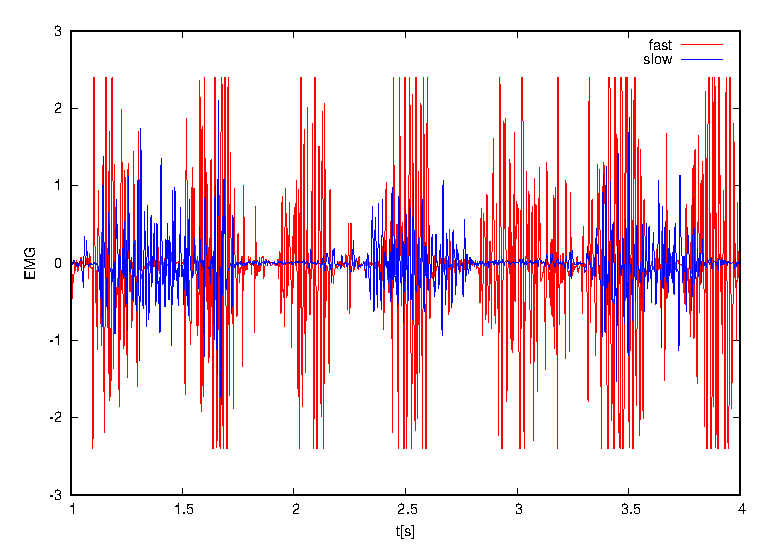
\includegraphics[width=10cm]{kndata1.eps}
%\caption{上腕二頭筋のEMG生データ}
%\label{kndata1}
%\end{center}
%\end{figure}
%
%\begin{figure}[htb]
%\begin{center}
%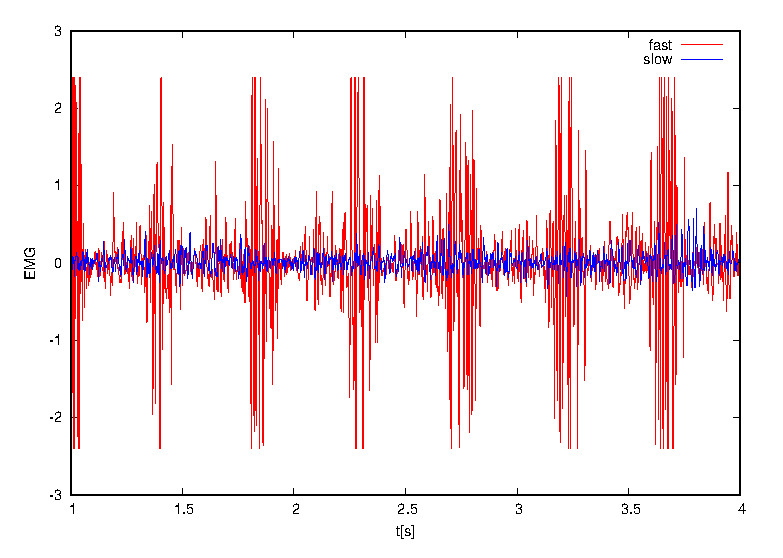
\includegraphics[width=10cm]{kndata2.eps}
%\caption{上腕三頭筋のEMG生データ}
%\label{kndata2}
%\end{center}
%\end{figure}
%
%\subsection{バンドパスフィルタ後}\label{kdata}
% \ref{ndata}のデータに\ref{s1}の処理を加えた結果を図\ref{kbdata1}、\ref{kbdata2}に示す。
%\begin{figure}[htb]
%\begin{center}
%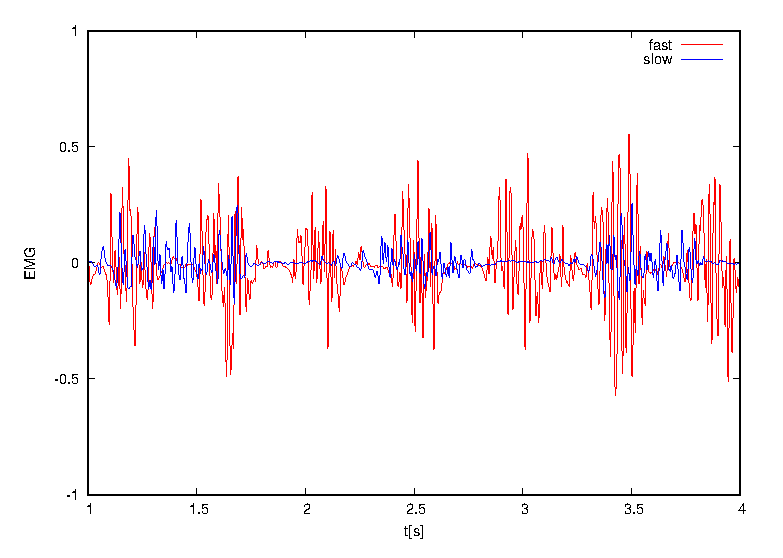
\includegraphics[width=10cm]{kbdata1.eps}
%\caption{上腕二頭筋のEMGBPF後}
%\label{kbdata1}
%\end{center}
%\end{figure}
%
%\begin{figure}[htb]
%\begin{center}
%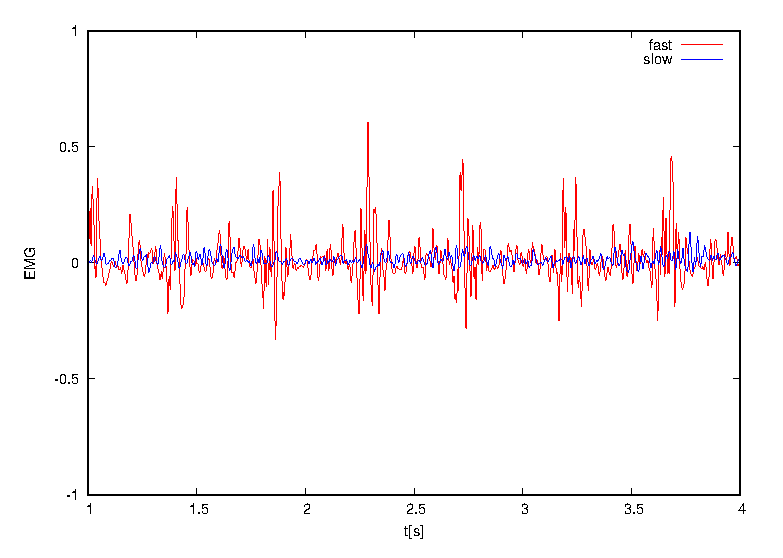
\includegraphics[width=10cm]{kbdata2.eps}
%\caption{上腕三頭筋のEMGBPF後}
%\label{kbdata2}
%\end{center}
%\end{figure}
%
%\newpage
%
%\subsection{整流化後}\label{adata}
% \ref{kdata}のデータを整流した結果を図\ref{kadata1}、\ref{kadata2}に示す。
%\begin{figure}[htb]
%\begin{center}
%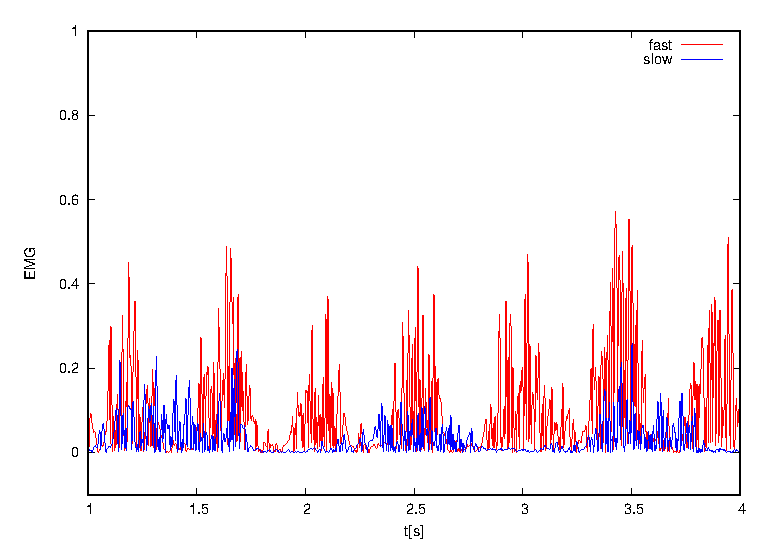
\includegraphics[width=10cm]{kadata1.eps}
%\caption{上腕二頭筋のEMG整流後}
%\label{kadata1}
%\end{center}
%\end{figure}
%
%\begin{figure}[htb]
%\begin{center}
%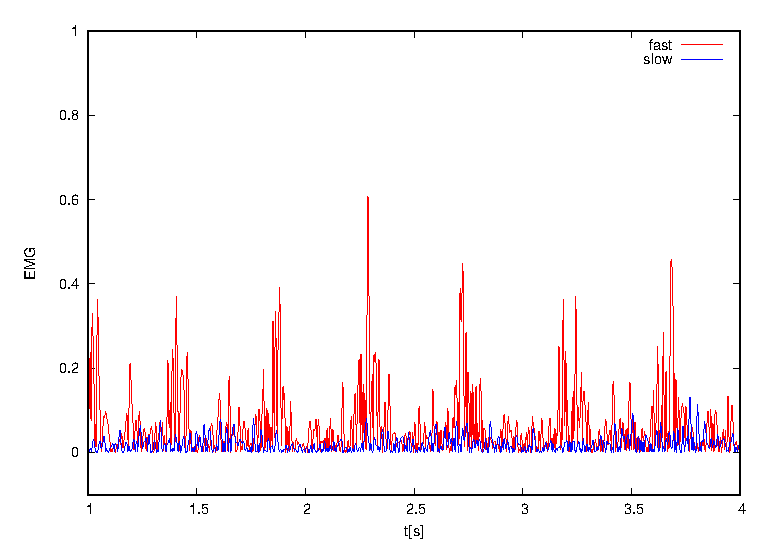
\includegraphics[width=10cm]{kadata2.eps}
%\caption{上腕三頭筋のEMG整流後}
%\label{kadata2}
%\end{center}
%\end{figure}
%
%\newpage
%
%\subsection{活動度}
% \ref{adata}のデータに\ref{s2}の処理を$\Delta T=50$で加えた結果を図\ref{kkdata1}、\ref{kkdata2}に示す。
%
%
%図\ref{kndata1}、\ref{kndata2}と図\ref{kkdata1}、\ref{kkdata2}を比較しても分かる通り、筋肉の活動の時間変化を観察しやすくなっている。例えば、図\ref{kkdata1}と図\ref{kkdata2}の赤いグラフの比較を行うと双対的に活動量が変化していることがわかる。
%
%
%
%\section{モーションキャプチャのデータ}
%\subsection{t-xデータ}
% 肩の動きの結果を図\ref{txm1}に、肘の動きを図\ref{txm2}に、手首の動きを図\ref{txm3}にそれぞれまとめた。また、以下に示すモーションキャプチャのデータは筋電と同様に速く動かした場合を赤と遅く動かした場合を青で示してある。
%\begin{figure}[htb]
%\begin{center}
%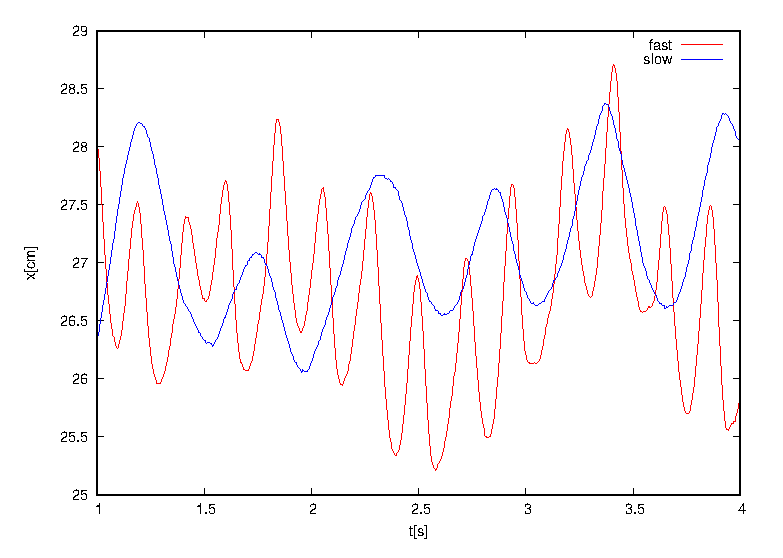
\includegraphics[width=10cm]{txm1.eps}
%\caption{肩の時間におけるx軸方向の動き}
%\label{txm1}
%\end{center}
%\end{figure}
%
%\begin{figure}[htb]
%\begin{center}
%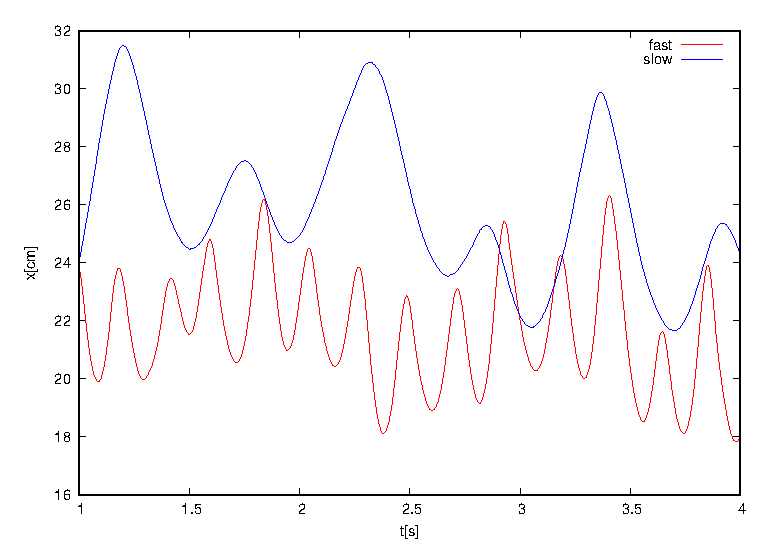
\includegraphics[width=10cm]{txm2.eps}
%\caption{肘の時間におけるx軸方向の動き}
%\label{txm2}
%\end{center}
%\end{figure}
%
%\begin{figure}[htb]
%\begin{center}
%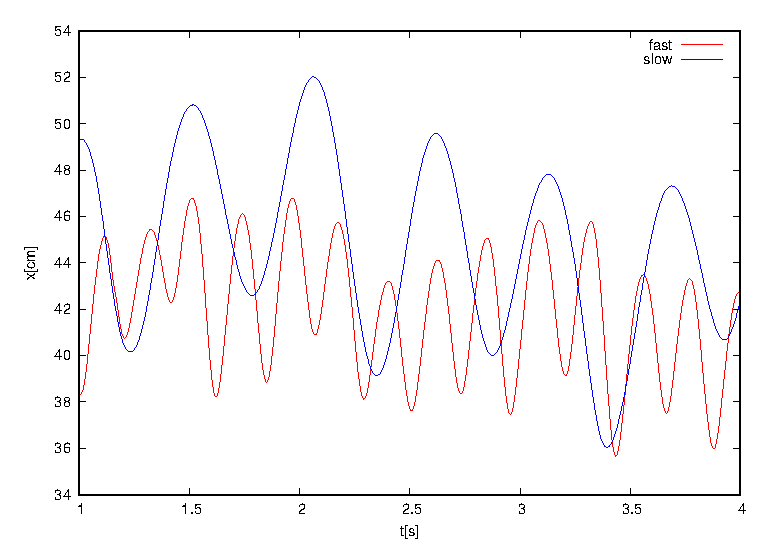
\includegraphics[width=10cm]{txm3.eps}
%\caption{手首の時間におけるx軸方向の動き}
%\label{txm3}
%\end{center}
%\end{figure}
%
%
%\subsection{t-yデータ}
% 肩の動きの結果を図\ref{tym1}に、肘の動きを図\ref{tym2}に、手首の動きを図\ref{tym3}にそれぞれまとめた。
%
%\begin{figure}[htb]
%\begin{center}
%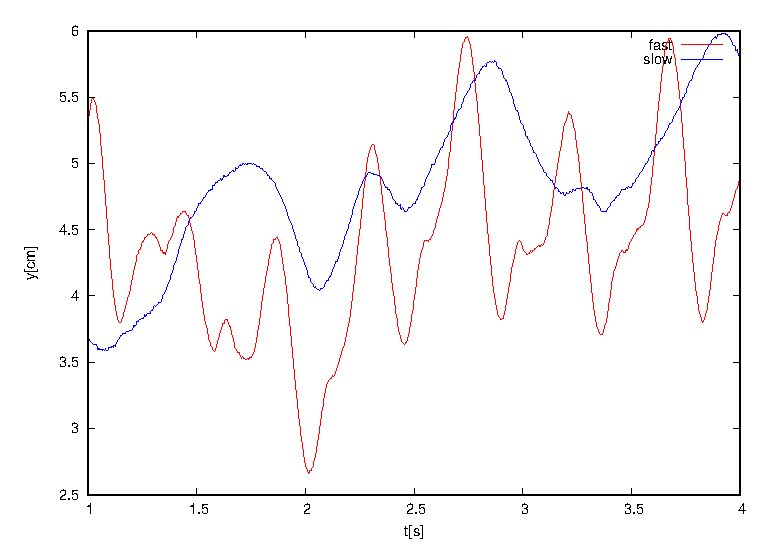
\includegraphics[width=10cm]{tym1.eps}
%\caption{肩の時間におけるy軸方向の動き}
%\label{tym1}
%\end{center}
%\end{figure}
%
%\begin{figure}[htb]
%\begin{center}
%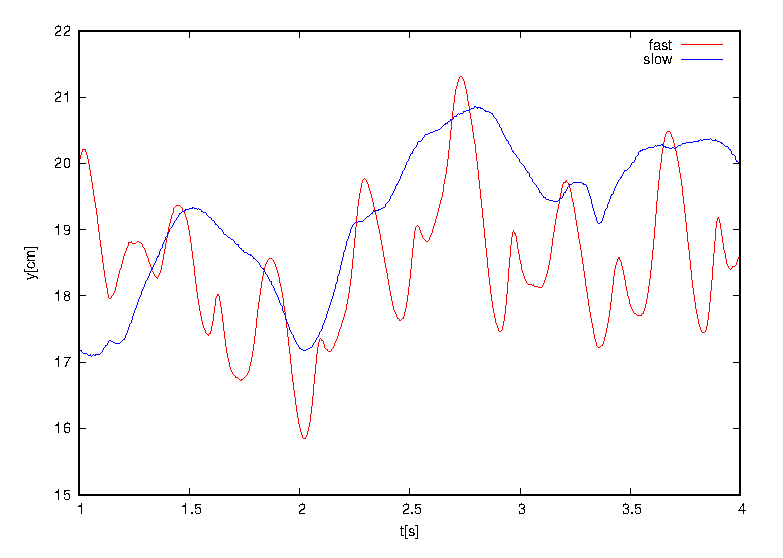
\includegraphics[width=10cm]{tym2.eps}
%\caption{肘の時間におけるy軸方向の動き}
%\label{tym2}
%\end{center}
%\end{figure}
%
%
%
%\clearpage
%
%\subsection{x-yデータ}
% x-yの関係性を図\ref{xym1}にまとめた。この際の体の位置関係は図\ref{karada}と同様である。
%
%
%
%
%\section{考察}
% 図\ref{tym3}より、1$\sim$4秒の3秒間にfastは7回、slowは3回手首を前後させていることから、それぞれその回数分屈筋運動していることがわかる。この動きに対し、図\ref{txm1}、\ref{txm2}、\ref{txm3}ではfastは13$\sim$14回、slowは5$\sim$6回左右に運動させていることがわかる。よって、1度屈筋運動をするのに、2度左右に移動させていることがわかる。また、図\ref{kkdata1}の活動量の上がるタイミングと図\ref{tym3}の前に手が出るタイミングが同じであることから、腕を伸ばすタイミングに上腕二頭筋を使用し、腕を曲げるタイミングに上腕三頭筋を使用していることがわかる。
%
%



\end{document}